\section*{Úvodní část}
Tento znalecký posudek byl vypracován na žádost zadavatele posudku.

\vspace{0.5cm}
\noindent
Jméno znalce: Martin Zlámal, Plzeň \\
Zadavatel: Pythagoras ze Samu, ostrov Samos

\vspace{0.5cm}
\noindent
Účel posudku: \textbf{Dokázat, že věta $a^2+b^2=c^2$ platí pro libovolný pravoúhlý trojúhelník.}

\section*{Nález}
Jednoduchým poskládáním čtyř libovolných pravoúhlých trojúhleníků lze se sestavit čtverec jehož jedna strana je dlouhá $a+b$:

\begin{figure}[h]
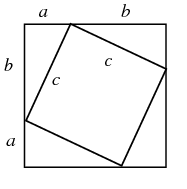
\includegraphics[scale=0.5]{prove.png}
\end{figure}

\noindent
Plocha každého ze čtyř trojúhelníků je rovna $\frac{1}{2}ab$ a plocha vnitřního čtverce je $c^2$. Z obrázku je patrné, že plocha velkého čtverce (vnějšího) je součet jednotlivých trojúhleníků a vnitřního čtverce, tedy:
\[S=4(\frac{1}{2}ab)+c^2\]
Platí také, že plocha velkého čtverce je rovna $(a+b)^2$. Tato plocha se logicky musí rovnat první variantě, tedy:
\[4(\frac{1}{2}ab)+c^2=(a+b)^2\]
Kdy po odstranění závorek dostáváme výraz:
\[2ab+c^2=a^2+2ab+b^2\]
Odstraněním společného výrazu na obou stranách rovnice $2ab$ získáváme původní výraz:
\[c^2=a^2+b^2\]
Plocha velkého čtverce je stále stejně velká nehledě na použitém postupu. Porovnáním dvou různých přístupů k výpočtu této plochy získáme vždy stejný výraz. Tuto úvahu lze provést pro libovolný pravoúhlý trojúhelník, neboť i v předchozím postupu bylo místo čísel použito symbolů $a$, $b$ a $c$.

\section*{Posudek}
Věta $a^2+b^2=c^2$ platí pro libovolný pravoúhlý trojúhelník.

\section*{Znalecká doložka}
Znalecký posudek jsem podal jako znalec jmenovaný rozhodnutím (ministra spravedlnosti) ze dne 12. 1. 2016. čj.: 123/4567. pro základní obor ŠKOLSTVÍ A KULTURA. odvětví Pedagogika. Znalecký úkon je zapsán pod poř. č. 123 - 4567/891011 znaleckého deníku. Znalečné a úhrada nákladů je vyúčtováno na základě samostatného účetního dokladu.

\vspace{0.5cm}
\noindent
Tento znalecký posudek se skládá ze dvou listů a úvodní strany. Znalecký posudek byl vyhotoven ve dvou stejných vyhotoveních.

\vspace{5cm}
\hfill .....................................\\
V Plzni dne 15. 3. 2017 \hfill Martin Zlámal
